\documentclass[class=book, crop=false, oneside, 12pt]{standalone}
\usepackage{standalone}
\usepackage{amsmath}
\usepackage{../../style}
\graphicspath{{./assets/images/}}

% arara: pdflatex: { synctex: yes, shell: yes }
% arara: latexmk: { clean: partial }
\begin{document}

\chapter{Legge di Gauss}

\section{Angolo solido}
%TODO In questa sezione e nelle prossime sarebbe meglio aggiungere un bel po di foto dal libro

\begin{figure}[h]
    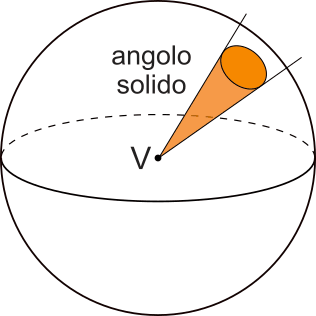
\includegraphics[scale=0.4]{angolo-solido}
    \centering
    \caption{}
\end{figure}

Sia \(d \Sigma\) un elemento di superficie, \(\overrightarrow{u}_n\) la sua normale e \(d \Sigma_0\) la sua funzione ortogonale a \(\overrightarrow{u}_r\), il versore del raggio uscente da un punto di osservazione \(0\). 
Si definisce angolo solido infinitesimo, la quantità
\begin{equation}
    d \Omega = \frac{d \Sigma \cos \alpha}{r^2} = \frac{d \Sigma_0}{r^2}
\end{equation}

L'angolo solido è l'estensione a tre dimensioni del concetto di angolo piano infinitesimo:
\begin{equation}
    d \theta = \frac{ds' \cos \alpha}{r} = \frac{ds}{r}
\end{equation}
La superficie \(d \Sigma_0\) è un elemento di calotta sferica e la sua area vale (nel sistema a coordinate polari)
\begin{equation} \label{misura_infinitesimo_angolo_solido}
    d \Omega = \frac{d \Sigma_0}{r^2} = \sin \theta d \theta d \phi
\end{equation}

La (\ref{misura_infinitesimo_angolo_solido}) esprime l'angolo solido sotto cui dal punto \(0\) si vede il contorno \(ABCD\) della superficie \(d \Sigma_0\): 
risulta che \(d \Omega\) non dipende dal raggio \(r\). 
Geometricamente, possiamo dire che l'angolo solido dà una misura della parte di spazio compresa entro un fascio di semirette uscenti da \(0\), così come l'angolo piano dà una misura della parte di piano compresa tra due semirette uscenti da \(0\).

Per una superficie finita l'angolo solido è dato dall'integrale
\begin{equation}
    \Omega \sin \theta d \theta d \phi
\end{equation}
che è un integrale doppio sulle variabili \(\theta\) e \(\phi\).

Se, a \(0\) costante, si fa variare \(\phi\) da zero a \(2 \pi\), abbiamo l'angolo solido sotto cui da \(0\) è vista la corona sferica infinitesima
\begin{equation}
    d \Omega = \sin \theta d \theta \int_0^{2 \pi} d \phi = 2 \pi \sin \theta d \theta
\end{equation}
Integrando da \(\theta_1\) a \(\theta_2\)
\begin{equation*}
    \Omega (\theta_1 , \theta_2) = 2 \pi \left(\cos \theta_1 - \cos \theta_2 \right)
\end{equation*}
In particolare se \(\theta_1 = 0\) e \(\theta_2 = \theta\)
\begin{equation}
    \Omega (\theta) = 2 \pi (1- \cos \theta)
\end{equation}
e infine, se \(\theta_2 = \pi\), abbiamo l'angolo solido sotto cui dal centro è vista tutta la superficie sferica, 
\begin{equation}
    \Omega = 4 \pi
\end{equation}

\section{Flusso del campo elettrostatico, Legge di Gauss}

\subsection{Definizione di flusso attraverso una superficie}

Consideriamo, una superficie \( d \Sigma\) in una regione in cui è definito un campo \(\overrightarrow{E}\) e orientiamola fissando il verso del versore della normale \(\overrightarrow{u}_n\). 
Si definisce flusso del campo \(\overrightarrow{E}\) attraverso la superficie \(d \Sigma\) la quantità scalare 
\begin{equation} \label{definizione_flusso}
    d \Phi (\overrightarrow{E}) = \overrightarrow{E} \cdot \overrightarrow{u}_n d \Sigma = E \cos \theta d \Sigma = E_n d \Sigma
\end{equation}

Il flusso attraverso una superficie finita \(\Sigma\), si ottiene suddividendo la superficie \(\Sigma\) in elementi infinitesimi di superficie \(d \Sigma_i\), calcolando per ciascuno di essi il flusso infinitesimo \(d \Phi (\overrightarrow{E}_i) = \overrightarrow{E}_i \cdot u_{i,n} d \Sigma_i\), 
e sommando gli infiniti contributi, procedura che porta ad un integrale di superficie:
\begin{equation}
    \Phi (\overrightarrow{E}) = \int_{\Sigma} = \overrightarrow{E} \cdot \overrightarrow{u}_n d \Sigma
\end{equation}
Se la superficie è chiusa, il flusso si scrive, con l'integrale di ciclo chiuso:
\begin{equation} \label{flusso_superficie_chiusa}
    \Phi (\overrightarrow{E}) = \oint_{\Sigma} = \overrightarrow{E} \cdot \overrightarrow{u}_n d \Sigma
\end{equation}

In questo caso è convenzione orientare la normale verso l'esterno. 
I contributi positivi all'integrale (\ref{flusso_superficie_chiusa}) sono quelli per cui \(E \cdot \overrightarrow{u}_n> 0\), dovuti a quelle zone dove anche \(\overrightarrow{E}\) punta verso l'esterno: essi rappresentano un flusso di \(\overrightarrow{E}\) \emph{uscente dalla superficie}. 
I contributi negativi provengono dalle zone in cui \(E \cdot \overrightarrow{u}_n < 0\), in cui cioè \(\overrightarrow{E}\) punta verso l'interno, e rappresentano un flusso di \(\overrightarrow{E}\) \emph{entrante}. 
Pertanto (\ref{flusso_superficie_chiusa}) dà \emph{il flusso netto attraverso la superficie chiusa}; se esso è nullo vuol dire che il flusso entrante eguaglia in modulo il flusso uscente.

\subsection{Legge di Gauss}

La legge di Gauss stabilisce che: 
il flusso del campo elettrostatico \(\overrightarrow{E}\) prodotto da un sistema di cariche attraverso una superficie chiusa è uguale alla somma algebrica delle cariche elettriche contenute all'interno della superficie, divisa per \(\epsilon_0\).
\begin{equation}
    \Phi (\overrightarrow{E}) = \oint \overrightarrow{E} \cdot \overrightarrow{u}_n d \Sigma = \frac{1}{\epsilon_0} (\Sigma_i q_i)_{int}
\end{equation}
La legge vale indipendentemente da come sono distribuite le cariche all'interno della superficie.
Si noti che il campo \(\overrightarrow{E}\) che compare nell'integrale del flusso è il campo risultante delle tre cariche.
\begin{equation}
    \Phi (\overrightarrow{E}) = \oint \overrightarrow{E} \cdot \overrightarrow{u}_n d \Sigma = \frac{1}{\epsilon_0} \int dq
\end{equation}
essendo l'integrale al terzo membro esteso a tutto il volume \(\tau\) racchiuso da \(\Sigma\).. 
In pratica, poi, l'integrale è esteso ai soli punti in cui c'è carica \(dp \neq 0\). 

Unificando la struttura dell'ultimo membro la legge di Gauss si presenta in maniera generale come:
\begin{equation}
    \Phi (\overrightarrow{E}) = \oint \overrightarrow{E} \cdot \overrightarrow{u}_n d \Sigma = \frac{q}{\epsilon_0}
\end{equation}

\section{Dimostrazione della legge di Gauss}

Prendiamo in esame il campo elettrostatico prodotto da una carica puntiforme \(q\), e calcoliamo il flusso attraverso l'elemento di superficie orientata utilizzando (\ref{definizione_flusso}):
\begin{equation*}
    d \Phi (\overrightarrow{E}) = \frac{q}{4 \pi \epsilon_0} \frac{\overrightarrow{u}_r \cdot \overrightarrow{u}_n d \Sigma}{r^2} = \frac{q}{4 \pi \epsilon_0} + \frac{d \Sigma \cos \theta}{r^2} = \frac{q}{4 \pi \epsilon_0} + \frac{d \Sigma_0 }{r^2}
\end{equation*}
dove \(d \Sigma_0\) è la proiezione di \(d \Sigma\) sul piano perpendicolare a \(\overrightarrow{u}_r\). 
Per definizione \(d \Sigma_0 / r^2\) è l'angolo solido \(d \Omega\) sotto cui è visto dalla carica \(q\) il contorno di \(d \Sigma\), per cui
\begin{equation}
    d \Phi (\overrightarrow{E}) = \frac{q}{4 \pi \epsilon_0} d \Omega
\end{equation}

Il flusso del campo elettrostatico \(\overrightarrow{E}\) di una carica puntiforme \(q\) dipende solo dall'angolo solido e non dalla superficie né dalla sua distanza dalla carica; ottengo quindi
\begin{equation*}
    d \Omega = \frac{d \Sigma_1 \cos \theta_1}{r_1^2} = \frac{d \Sigma_{1,0}}{r_1^2} = \frac{d \Sigma_2 \cos \theta_2}{r_2^2} = \frac{d \Sigma_{2,0}}{r_2^2}
\end{equation*}

Il flusso attraverso una superficie finita è dato da
\begin{equation} \label{flusso_superficie_finita}
    \Phi (\overrightarrow{E}) = \int_{\Sigma} \overrightarrow{E} \cdot \overrightarrow{u}_n d \Sigma = \frac{q}{4 \pi \epsilon_0} \int d \Omega = \frac{q}{4 \pi \epsilon_0} \Omega 
\end{equation}
con \(\Omega\), angolo solido sotto cui è visto il contorno della superficie \(\Sigma\), dalla carica \(q\).

\subsection{Carica Interna}

Se la carica è interna, tutti i contributi \(\overrightarrow{E} \cdot \overrightarrow{u}_n d \Sigma\) si sommano in quanto hanno sempre lo stesso segno in qualsiasi punto di \(\Sigma\), e applicando (\ref{flusso_superficie_chiusa}) abbiamo
\begin{equation} \label{flusso_carica_interna}
    \Phi (\overrightarrow{E}) = \frac{q}{4 \pi \epsilon_0} \oint d \Omega = \frac{q}{4 \pi \epsilon_0} 4 \pi = \frac{q}{\epsilon_0}
\end{equation}
infatti l'angolo solido totale sotto cui è vista una superficie chiusa qualunque da un punto all'interno è \(4 \pi\).

\subsection{Carica Esterna}

Se invece la carica è esterna alla superficie chiusa, consideriamo, un cono elementare che sottende l'angolo solido \(d \Omega\) e che stacca sulla superficie chiusa due elementi \(d \Sigma_1\) e \(d \Sigma_2\);
l'orientazione della normale è tale che su \(d \Sigma_1 \overrightarrow{E} \cdot \overrightarrow{u}_n <0 \) e su \(d \Sigma_2 \overrightarrow{E} \cdot \overrightarrow{u}_n <0\). 

I flussi attraverso i due elementi sono: 
\begin{equation*}
    d \Phi_1 (\overrightarrow{E}) = \overrightarrow{E}_1 \cdot \overrightarrow{u}_n d \Sigma_1 = - \frac{q}{4 \pi \epsilon_0} d \Omega
\end{equation*}
\begin{equation*}
    d \Phi_2 (\overrightarrow{E}) = \overrightarrow{E}_2 \cdot \overrightarrow{u}_n d \Sigma_2 = \frac{q}{4 \pi \epsilon_0} d \Omega = - d \Phi_1 (E)
\end{equation*}
\begin{equation*}
    \implies d \Phi_1 (\overrightarrow{E}) + d \Phi_2 (\overrightarrow{E}) = 0
\end{equation*}

Integrando su tutta la superficie ottengo:
\begin{equation} \label{flusso_carica_esterna}
    d \Phi_1 (\overrightarrow{E}) = \oint \overrightarrow{E} \cdot \overrightarrow{u}_n d \Sigma
\end{equation}

Posso riassumere (\ref{flusso_carica_interna}) e (\ref{flusso_carica_esterna}): \emph{il flusso totale attraverso una superficie chiusa del campo elettrostatico di una carica puntiforme \(q\) vale \(q /\epsilon_0\) se la carica è interna alla superficie, vale zero se la carica è esterna}.

\subsection{Cariche puntiformi e cariche uniformemente distribuite}

Il risultato enunciato si estende al caso di più cariche puntiformi, attraverso il principio di sovrapposizione e la proprietà additiva degli integrali: 
il flusso attraverso una superficie chiusa del campo elettrostatico \(\overrightarrow{E}\) generato da un sistema discreto di cariche è dato da
\begin{equation*}
    \Phi (\overrightarrow{E}) = \oint \overrightarrow{E} \cdot \overrightarrow{u}_n d \Sigma = \oint (\Sigma_i \overrightarrow{E}_i) \cdot \overrightarrow{u}_n d \Sigma = \Sigma_i \oint \overrightarrow{E}_i \cdot \overrightarrow{u}_n d \Sigma
\end{equation*}
Ciascun integrale vale \(q_i / \epsilon_0\) se la carica è contenuta all'interno della superficie e vale zero se la carica è esterna.
\begin{equation} \label{flusso_cariche_puntiformi}
    \Phi (\overrightarrow{E}) = \frac{1}{\epsilon_0} (\Sigma_i q_i)_{int}
\end{equation}
essendo la somma estesa a tutte e sole le cariche poste all'interno della superficie \(\Sigma\).

Nel caso più generale in cui il campo sia generato da una distribuzione continua di cariche, la (\ref{flusso_cariche_puntiformi}) diviene
\begin{equation} \label{flusso_distribuzione_continua}
    \Phi (\overrightarrow{E}) = \frac{1}{\epsilon_0} \int_{\tau} dq
\end{equation}
dove l'integrale, esteso al volume \(\tau\) racchiuso dalla superficie \(\Sigma\), rappresenta sempre la carica totale contenuta all'interno di \(\Sigma\).

\section{Applicazioni teorema di Gauss}

La legge di Gauss diventa uno strumento molto efficace per determinare il campo elettrostatico E nei casi in cui la distribuzione di carica che genera il campo elettrostatico presenti un elevato grado di simmetria (sferica, cilindrica, piana).
In queste condizioni di norma è facile individuare a priori l'andamento delle linee di forza e trovare di conseguenza delle superficie chiuse \(\overrightarrow{E}\) nei cui punti il campo elettrostatico è parallelo o ortogonale alla superficie stessa, per cui i contributi \(\overrightarrow{E} \cdot \overrightarrow{u}_x d \Sigma\) o sono nulli, o si scrivono semplicemente \(E d \Sigma\). 
Se inoltre si può dedurre che il modulo del campo elettrostatico è costante in una zona di area \(\Sigma^{\prime}\) in cui \(\overrightarrow{E}\) è parallelo a \(\overrightarrow{u}_n\), la legge di Gauss assume la forma:
\begin{equation*}
    \Phi (\overrightarrow{E}) = \oint \overrightarrow{E} \cdot \overrightarrow{u}_n d \Sigma = E \Sigma = \frac{q}{e_0}
\end{equation*}
da cui si trova subito il modulo del campo elettrostatico: 
\begin{equation*}
    E = \frac{q}{e_0 \Sigma^{\prime}}
\end{equation*}
dove \(q\) è la carica posta all'interno della superficie chiusa \(\Sigma\). 

\subsection{Campo elettrostatico di una distribuzione sferica superificale di carica}
% TODO aggiungere foto del caso
Una carica \(q\) è distribuita con densità superficiale costante \(\sigma\) su una superficie sferica di raggio \(R\).  
Nel punto \(P\) distante \(r > R\) dal centro \(\overrightarrow{E}\) è certamente radiale, in quanto è dovuto alla somma di contributi a due a due simmetrici, eguali in modulo, la cui risultante è radiale; se così non fosse vorrebbe dire che \(\sigma\) non è uniforme.  
In qualsiasi altro punto che ha la stessa distanza di \(P\) dal centro la situazione è la stessa. 
Ciò significa che il campo ha modulo costante su una superficie sferica di raggio \(r\), è  ortogonale a questa e ha verso uscente o entrante a seconda del segno della carica.


Applicando ad una superficie sferica \(\Sigma\); di raggio \(r > R\):
\begin{equation*}
    \Phi (\overrightarrow{E}) = \oint \overrightarrow{E}(r) \overrightarrow{u}_r \cdot \overrightarrow{u}_n d \Sigma = \overrightarrow{E}(r) \oint d \Sigma = E(r) 4 \pi r^2 = \frac{q}{e_0}
\end{equation*}
con \(q = 4 \pi R^2 \Sigma\). Ottengo quindi:
\begin{equation*}
    \overrightarrow{E}(r) = \frac{q}{4 \pi \epsilon_0 r^2} = \frac{\sigma R^2}{\epsilon_0 r^2}
\end{equation*}
\begin{equation*}
    \overrightarrow{E} = \frac{q}{4 \pi \epsilon_0 r^2} \overrightarrow{u}_r
\end{equation*}

Il campo all'esterno di una distribuzione superficiale sferica uniforme di carica è eguale a quello di una carica puntiforme di egual valore posta nel centro della superficie sferica; a parità di carica esso non dipende dal raggio della distribuzione.

All'interno della superficie sferica valgono le stesse ragioni di simmetria per cui il campo dovrebbe essere radiale e il flusso attraverso una qualsiasi superficie sferica \(\Sigma^{\prime}\) di raggio \(r < R\) dovrebbe valere \(E \Sigma^{\prime}\).
D'altra parte all'interno non c'è carica, il flusso attraverso \(\Sigma^{\prime}\) è nullo e quindi deve essere \(E = 0\) per \(r < R\): all'interno di una distribuzione superficiale sferica uniforme il campo elettrostatico è nullo.
% TODO aggiungere grafici
\subsection{Campo elettrostatico prodotto da una sfera uniformemente carica}
% TODO aggiungere foto del caso
Una carica \(q\) è distribuita con densità spaziale \(\rho\) uniforme nel volume di una sfera di raggio \(R\).  
Il ragionamento basato sulla simmetria sferica utilizzato precedentemente, è valido anche adesso per \(r > R\) e possiamo subito dire che il campo all'esterno di una sfera uniformemente carica vale
\begin{equation*}
    \overrightarrow{E} = \frac{q}{4 \pi \epsilon_0 r^2}\overrightarrow{u}_r = \frac{\rho R^3}{3 \epsilon_0 r^2} \overrightarrow{u}_r
\end{equation*}
con 
\begin{equation*}
    q = \frac{4}{3} \pi R^3 \rho
\end{equation*}
è come se la carica fosse concentrata nel centro della sfera.  

Ne segue che il modulo del campo elettrostatico a distanza \(r < R\) dal centro vale
\begin{equation*}
    E = \frac{q^{\prime}}{4 \pi \epsilon_0 r^2} = \frac{q r }{4 \pi \epsilon_0 R^3} = \frac{\rho r}{3 \epsilon_0}
\end{equation*}
In conclusione, il campo cresce linearmente dal valore zero assunto nel centro della sfera al valore \(\rho R / 3 \epsilon_0 = q / 4 \pi \epsilon_0 R^2\) assunto sulla superficie della sfera; all'esterno esso decresce con il quadrato della distanza dal centro.

Il potenziale della sfera è dato da \(V = q / 4 \pi \epsilon_0 r\) e in particolare vale
\begin{equation*}
    V(R) = \frac{q}{4 \pi \epsilon_0 R} = \frac{\rho R^2}{3 \epsilon_0}
\end{equation*}
sulla superficie della sfera. All'interno
\begin{equation*}
    V(R) - V(r) = - \int_r^R \overrightarrow{E} \cdot d \overrightarrow{s} = - \int_r^R \frac{\rho r}{3 \epsilon_0} dr = - \frac{\rho}{6 \epsilon_0} (R^2 - r^2)
\end{equation*}
\begin{equation*}
    \implies V(r) = \frac{\rho}{6 \epsilon_0} (3 R^2 - r^2) = \frac{q}{8 \pi \epsilon_0 R} \left(3 - \frac{r^2}{R}\right)
\end{equation*}
% TODO add grafici
\subsection{Campo elettrostatico di un cilindro uniformemente carico}

Una distribuzione spaziale continua e uniforme di carica ha forma cilindrica di raggio \(R\); la lunghezza del cilindro è molto grande (al limite infinito) rispetto a \(R\) 

La simmetria cilindrica del problema suggerisce che il campo elettrostatico sia diretto in ogni punto ortogonalmente all'asse del cilindro formato dalla carica e sia costante su ogni superficie cilindrica coassiale di raggio \(r\).
Per applicare la legge di Gauss consideriamo una scatola cilindrica \(\Sigma\); di raggio \(r > R\) e altezza \(h\).

Il flusso di \(\overrightarrow{E}\) attraverso le basi di \(\Sigma\); è nullo in quanto il campo è parallelo alle basi e quindi ortogonale a \(\overrightarrow{u}_n\). 
Il flusso attraverso la superficie laterale, che per quanto detto coincide con il flusso totale attraverso \(\Sigma\), vale
\begin{equation*}
    \Phi(E) = E \Sigma = 2 \pi r h E = \frac{q}{\epsilon_0}
\end{equation*} 
La carica contenuta entro \(\Sigma\) è 
\begin{equation*}
    q = \int \rho d \tau = \rho \pi R^2 h = \lambda h
\end{equation*}
definendo
\begin{equation*}
    \lambda = \rho \pi R^2 = \frac{q}{h}
\end{equation*}
la carica contenuta in un cilindro di raggio \(R\) e altezza unitaria.

Quindi
\begin{equation*}
    \Phi(\overrightarrow{E}) = 2 \pi r h E = \frac{\lambda h}{\epsilon_0} 
\end{equation*}
\begin{equation*}
    E = \frac{\lambda}{2 \pi \epsilon_0 r}
\end{equation*}

La d.d.p. tra due qualsiasi superficie equipotenziali, che sono superficie cilindriche coassiali di raggi \(r_1\) e \(r_2\), con \(r_2 > r_1\) è: 
\begin{equation*}
    V(r_2) - V(r_1) = - \int_{r_1}^{r_2} E d r = - \int_{r_1}^{r_2} \frac{\lambda}{2 \pi \epsilon_0 r} d r = - \frac{\lambda}{2 \pi \epsilon_0} \ln \frac{r_2}{r_1}
\end{equation*}
rispetto al bordo \(r >> R\)
\begin{equation*}
    V(r_2) - V(r_1) = - \frac{\lambda}{2 \pi \epsilon_0} \ln \frac{r}{R}
\end{equation*}

I risultati trovati valgono anche per un sottile filo rettilineo molto lungo, su cui è depositata una carica distribuita con densità uniforme \(\lambda\).

\subsection{Campo elettrostatico di un piano indefinito uniformemente carico}

Una carica è distribuita con densità superficiale \(\sigma\) su un piano indefinito.  
Sempre in base a ragionamenti di simmetria si deduce che il campo elettrostatico è ortogonale al piano su cui è distribuita la carica e ha versi opposti dalle due parti (cioè è sempre uscente o sempre entrante).
Come superficie a cui applicare la legge di Gauss scegliamo una scatola cilindrica con le basi, di area \(\Sigma\), parallele al piano, così che il flusso attraverso le basi è \(2 E \Sigma\); mentre quello attraverso la superficie laterale è nullo.

All'interno della scatola c'è la carica \(q = \sigma \Sigma\): e Quindi
\begin{equation*}
    \Phi(\overrightarrow{E}) = 2 E \Sigma = \frac{\sigma \Sigma}{\epsilon_0} \implies E = \frac{\sigma}{2 \epsilon_0}
\end{equation*}

Vettorialmente, dato \(x\) un asse ortogonale al piano,
\begin{equation*}
    E_1 = E(x > 0 ) = \frac{\sigma}{2 \epsilon_0} \overrightarrow{u}_x
\end{equation*}
\begin{equation*}
    E_2 = E(x < 0 ) = - \frac{\sigma}{2 \epsilon_0} \overrightarrow{u}_x
\end{equation*}
nel passaggio attraverso la superficie carica il campo elettrostatico è discontinuo e ottengo che nel passaggio
\begin{equation*}
    E_1 - E_2 = \frac{\sigma}{2 \epsilon_0} \overrightarrow{u}_x - \frac{- \sigma}{2 \epsilon_0} \overrightarrow{u}_x = \frac{\sigma}{\epsilon_0} \overrightarrow{u}_x
\end{equation*}

La differenza di potenziale elettrostatico tra due punti distanti \(x_1\) e dal piano, con \(x_2 > x_1\) è 
\begin{equation*}
    V(x_2) - V(x_1) = - \int_{x_1}^{x_2} E dx = - \frac{\sigma}{2 \epsilon_0} (x_2 - x_1)
\end{equation*}

\end{document}